% Slide 正文均使用英文
\section{Introduction}

% 我的简介
\begin{frame}[fragile]{\emoji{bust-in-silhouette} Biography}
	\begin{center}
		\begin{itemize}
			\item \textbf{Baolin Zhu} (\emoji{bowling} @bowling233)
			\item (with Eric) Leader of ZJUSCT
			\item \textbf{Research Interests}: Arch/OS, Three Pillars (Compute, Network and Storage)
		\end{itemize}
		\begin{tikzpicture}
			% Timeline base line
			\draw[thick, gray] (0,0) -- (10.5,0);

			% Node 0: CKC AGC
			\fill[blue] (1.5, 0) circle (0.1);
			\draw[gray] (1.5, 0) -- (1.5, 0.5);
			\node at (1.5, 1) {
\includegraphics[width=0.8cm]{day8_pm/img/bio-ckcagc}};
			\node[font=\bfseries\small] at (1.5, 2) {CKC AGC};
			\node[font=\footnotesize, gray] at (1.5, -0.5) {Freshman};

			% Node 1: ZJUSCT
			\fill[blue] (4.0, 0) circle (0.1);
			\draw[gray] (4.0, 0) -- (4, 0.5);
			\node at (4.0, 1) {
\includegraphics[width=0.8cm]{day8_pm/img/bio-zjusct}};
			\node[font=\bfseries\small] at (4.0, 2) {ZJUSCT};
			\node[font=\footnotesize, gray] at (4.0, -0.5) {Sophomore};

			% Node 2: RC4ML Lab
			\fill[blue] (6.5, 0) circle (0.1);
			\draw[gray] (6.5, 0) -- (6.5, 0.5);
			\node at (6.5, 1) {
\includegraphics[width=0.8cm]{day8_pm/img/bio-rc4ml}};
			\node[font=\bfseries\small] at (6.5, 2) {RC4ML Lab};
			\node[font=\footnotesize, gray] at (6.5, -0.5) {Junior};

			% Node 3: Tencent
			\fill[blue] (9.0, 0) circle (0.1);
			\draw[gray] (9.0, 0) -- (9.0, 0.5);
			\node at (9.0, 1) {
\includegraphics[width=0.8cm]{day8_pm/img/bio-csig}};
			\node[font=\bfseries\small] at (9.0, 2) {Tencent CSIG};
			\node[font=\footnotesize, gray] at (9.0, -0.5) {Junior};

		\end{tikzpicture}
	\end{center}
\end{frame}

% 为什么学习 C++ 并行编程:减轻心智负担
\begin{frame}[fragile]{\emoji{question} Why C++ Concurrency?}
	Reducing cognitive overhead for \textbf{application-level} (rather than systems-level) programming.
	\begin{itemize}
		\item Object-Oriented Programming (OOP) \& Encapsulation
		\item Resource Management \& RAII: Smart pointers
		\item Templates \& Generic Programming
		\item Standard Template Library (STL) \& Abstractions
		\item Safer Concurrency Models
		\item Enhanced Type Safety \& Expressiveness: References, Function Overloading, and Lambdas
	\end{itemize}
\end{frame}

% 本节课的参考教材
\begin{frame}[fragile]{\emoji{books} Textbook}

	\begin{columns}
		\begin{column}{0.4\textwidth}
			\begin{center}
				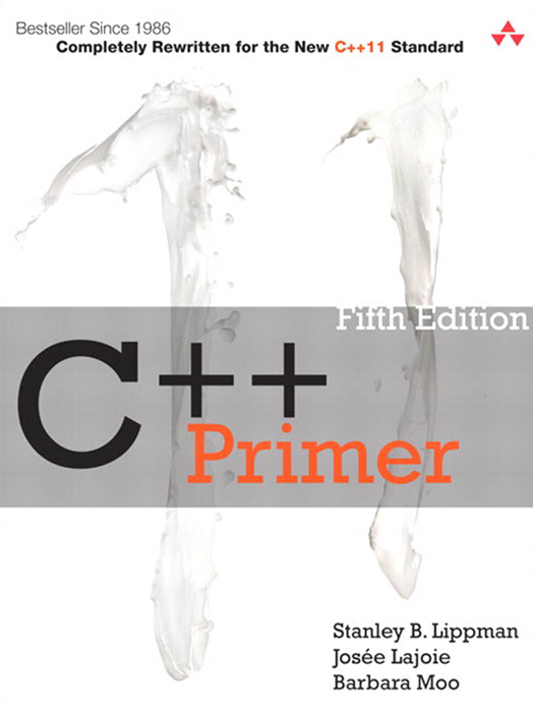
\includegraphics[width=0.8\textwidth]{day8_pm/img/1-cppprimer}
			\end{center}

		\end{column}
		\begin{column}{0.6\textwidth}
			\begin{itemize}
				\item \textbf{Title}: C++ Primer (Fifth Edition)
				\item \textbf{Authors}: Stanley B. Lippman, Josée Lajoie, and Barbara E. Moo
				\item \textbf{Publisher}: Addison-Wesley Professional
			\end{itemize}
		\end{column}
	\end{columns}
\end{frame}

\begin{frame}[fragile]{\emoji{books} Textbook}

	\begin{columns}
		\begin{column}{0.4\textwidth}
			\begin{center}
				
\includegraphics[width=0.8\textwidth]{day8_pm/img/1-ccia}
			\end{center}

		\end{column}
		\begin{column}{0.6\textwidth}
			\begin{itemize}
				\item \textbf{Title}: C++ Concurrency in Action (Second Edition)
				\item \textbf{Authors}: Anthony Williams
				\item \textbf{Publisher}: Manning Publications
			\end{itemize}
		\end{column}
	\end{columns}
\end{frame}

% Tips:遇到 C/C++ 语法问题,去 CPPREFERENCE 查找
\begin{frame}[fragile]{\emoji{light-bulb} Tips}
	\begin{itemize}
		\item \textbf{C/C++ Reference}: Use \textcolor{blue}{\href{https://en.cppreference.com/}{cppreference}} for syntax and library functions
		\item \textbf{Compiler Documentation}: Check your compiler's documentation for specific features and extensions (Example: \textcolor{blue}{\href{https://gcc.gnu.org/onlinedocs/gcc/Attributes.html}{GCC Attributes}})
		\item \textbf{Online Communities}: Engage with communities like Stack Overflow for troubleshooting and best practices
	\end{itemize}
\end{frame}

% Tips:关于 HPC 学习:适应系统性学习的思维方式的同学,需要适应点状式学习的思维方式
\begin{frame}[fragile]{\emoji{light-bulb} Systematic vs. Problem-Driven Learning}
	\scriptsize
	\begin{columns}
		\begin{column}{0.5\textwidth}
			\textbf{Systematic Learning}
			\begin{itemize}
				\item Builds a structured knowledge network
				\item Driven by internal logic of disciplines
				\item Strong foundation, long-term benefits
				\item Limitation: Time-consuming, less adaptive
			\end{itemize}
		\end{column}
		\begin{column}{0.5\textwidth}
			\textbf{Problem-Driven Learning}
			\begin{itemize}
				\item Focuses on solving specific problems
				\item Knowledge acquisition is modular and need-based
				\item Quick results, highly focused
				\item Limitation: Fragmented knowledge, less depth
			\end{itemize}
		\end{column}
	\end{columns}
	\vspace{0.5cm}
	\textbf{Key Insight:} Effective learners adaptively combine both approaches, leveraging systematic learning for foundational understanding and problem-driven learning for practical application.
	%\normalsize
\end{frame}

% 本节课的内容大纲
\begin{frame}[fragile]{\emoji{book} Outline}
	\begin{enumerate}
		\item \textbf{C++ Quick Start}
		      \begin{itemize}
			      \item Key differences between C++ and C
			      \item Object-oriented programming
			      \item Containers and Algorithms
		      \end{itemize}
		\item \textbf{C++ Concurrency Overview}
		      \begin{itemize}
			      \item Comparison: OpenMP, MPI, C++ threads
			      \item Thread lifecycle management
		      \end{itemize}
		\item \textbf{Shared Data Synchronization}
		      \begin{itemize}
			      \item From C mutexes to C++ RAII locks
			      \item Deadlock prevention strategies
		      \end{itemize}
		\item \textbf{Producer-Consumer Model}
		      \begin{itemize}
			      \item Condition variables and thread-safe queues
			      \item Practical implementation
		      \end{itemize}
		\item \textbf{Summary and Framework Selection}
		      \begin{itemize}
			      \item Comprehensive comparison and use cases
			      \item Monte Carlo π calculation example
		      \end{itemize}
	\end{enumerate}
\end{frame}

% 预修要求:C 语言,否则请先跳过本节课,补习 C 语言基础
\begin{frame}[fragile]{\emoji{warning} Prerequisites}
	\begin{itemize}
		\item \textbf{C Language Proficiency}: Basic understanding of C syntax and concepts
		\item \textbf{Familiarity with Pointers}: Understanding of pointers, memory management, and basic data structures
		\item \textbf{Basic Programming Constructs}: Loops, conditionals, functions, and arrays
	\end{itemize}
\end{frame}
